\subsection{Idee}
Arduinos können analoge Werte digitalisieren und sind sehr einfach zu handhaben und die Programmierung ist schnell zu erlernen. Wir haben bipolare Geschwindigkeitsaufnehmer, die eine Spannung abgeben, die proportional zur Bodengeschwindigkeit ist -- für entgegengesetzte Bewegungen ist die Spannung negativ. Der Arduino kann nur positive Spannungen verarbeiten, vorab muss demnach eine Schaltung entwickelt werden, die einen Offset auf das Signal gibt. Die Spannung darf (je nach Arduino-Typ)  3,3 V oder 5,0 V nicht überschreiten. Entgegen der Spezifikation konnten mit den Geophonen allerdings niemals Signale produziert werden, deren Amplitude den Eingangsbereichs der Arduinos überfordert hätten. Das Problem reduzierte sich daher darauf, nur Signale mit positiven Spannungen zu liefern. Eine klassische Gleichrichterschaltung konnten mit den vorhanden Bauteilen nicht realisiert werden, da nicht genug normale Dioden verfügbar waren. Zener-Dioden sind für diesen Zweck nicht geeignet, an LEDs ist der Spannungsabfall in Durchlassrichtung zu groß. Letztlich konnte eine Schaltung entwickelt werden, mit welche das Wechselspannungssignal der Geophone aufgeteilt wurde. 

\subsection{Einsortieren}
Zunächst muss eine Schaltung für einen Kanal entwickelt und getestet werden. Sollte das funktionieren, lässt sich überprüfen wie viele Sensoren verwendet werden können. Mit drei oder mehr sollte eine grobe Ortung in zwei Dimensionen möglich sein.

\subsection{Schaltung}
\begin{figure}
\centering
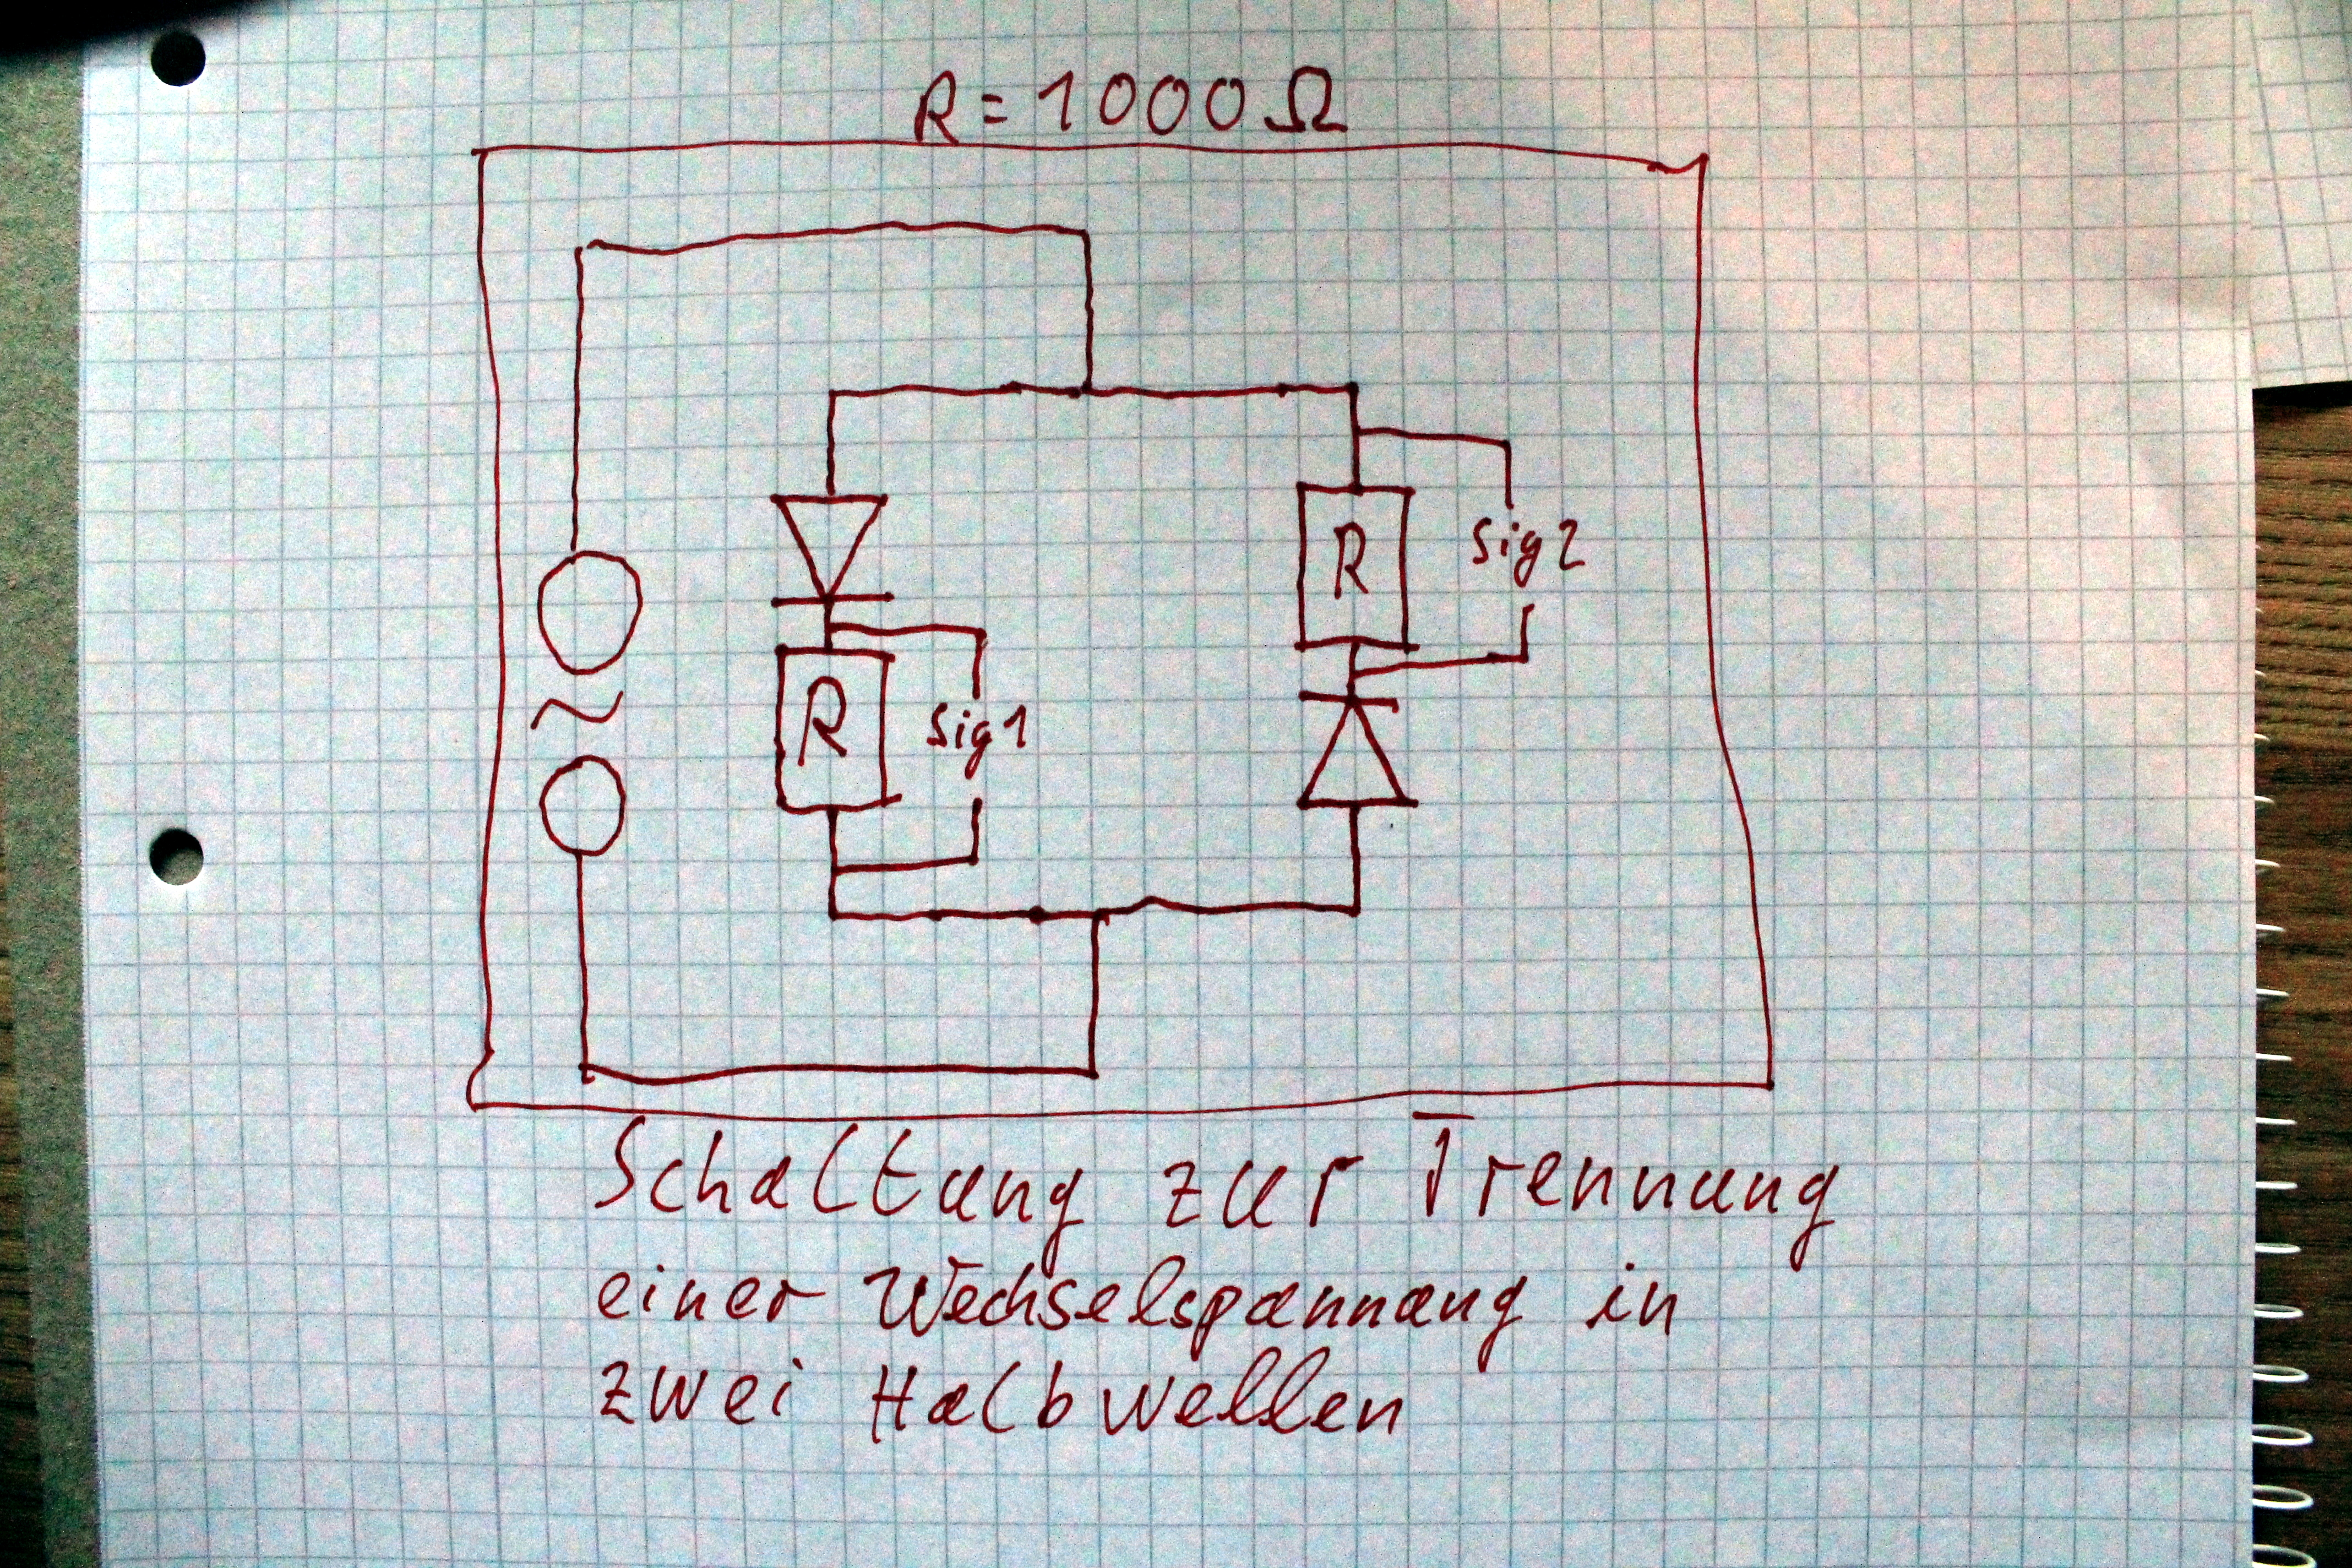
\includegraphics[width=\textwidth]{figs/geophone/skizze_schaltung}
\end{figure}

\begin{figure}
\centering
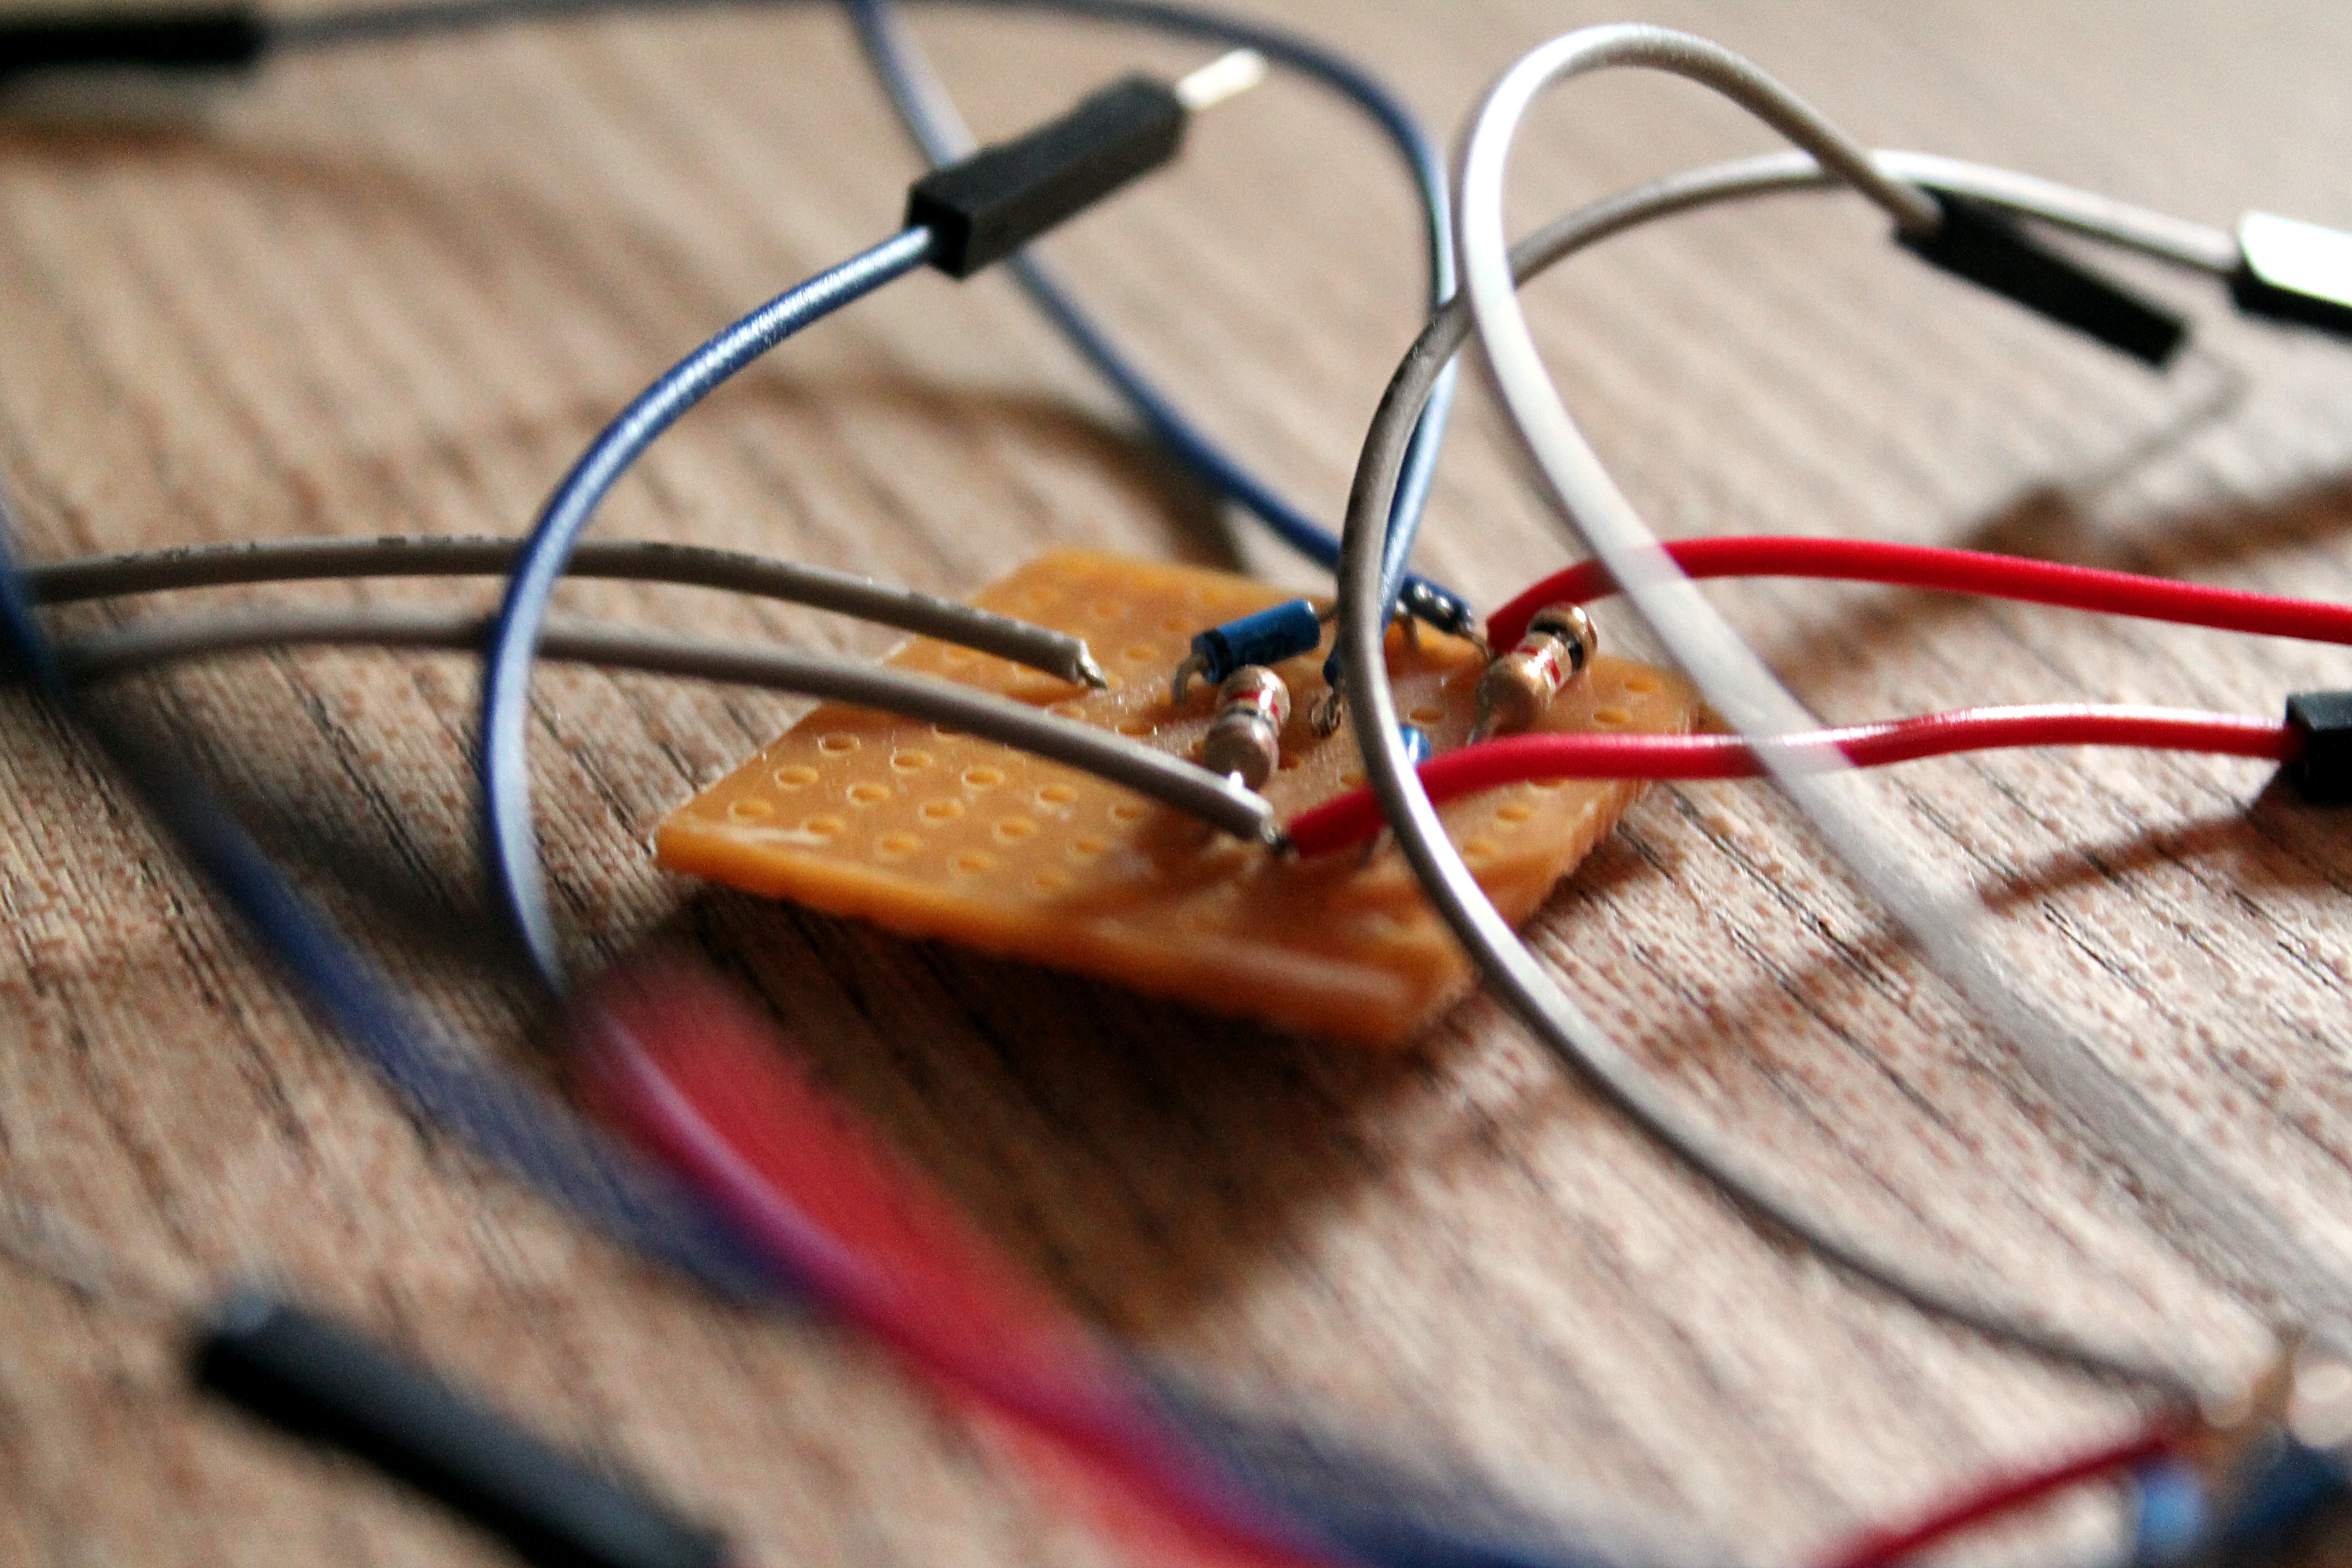
\includegraphics[width=\textwidth]{figs/geophone/schaltung}
\end{figure}

Die Schaltung, die letztlich verwandt wurde besteht aus zwei Widerständen und zwei Dioden. Der Widerstandswert wurde so groß wie möglich gewählt und dient dazu, die Signale an der richten Stelle abgreifen zu können. Die Dioden blockieren in jedem Parallelkreis jeweils eine Stromflussrichtung. Durch Wahl der Polung kann jede Halbwelle positiv oder negativ auf den Arduino gegeben werden. Eine Spannungsbegrenzung ist durch diese Schaltung nicht möglich.

\subsection{Auswertung}
Die Gephone liefern analoge Spannungssignale. Zur Auswertung müssen diese digitalisiert und an einen Rechner weitergeleitet werden. Die beiden vorhanden Arduinos stellen diese Funktionalität prinzipiell bereit. Ein kurzes Arduinoprogramm konnte schnell entwickelt werden um sämtliche Eingänge auszulesen und zu digitalisieren. Das Programm ist mit wenig Code realisierbar, allerdings gibt es Unklarheiten bezüglich der internen Vorgänge im Arduino. Beispielsweise ist die Samplingfrequenz die genutzt wird unklar. Über das Internet konnten kurzfristig zahlreiche Codebeispiele eingesehen werden. Umfangreicher war hingegen die weitere Auswertung am Rechner. Diese sollte in Python implementiert werden. Die Ausgabe der Signale in einem Diagramm war unproblematisch und funktioniert in Echtzeit. Als schwieriger erwies sich die Bestimmung der Laufzeitdifferenzen. Zunächst war unklar wie überhaupt auf ein Signal getriggert werden kann und welche Signale der drei genutzten Geophone zu einem Ereignis zu zuordnen ist. Die Bestimmung des Orts einer Ereignisses aus den relativen Laufzeitdifferenzen dreier Geophone ist darüber hinaus kein triviales Problem. Es wurden mehrere Lösungsansätze besprochen, jedoch nicht ausprobiert.

\subsection{Protokoll}
Stand 05.09.13
\begin{itemize}
	\item Induktivitäten mit Widerständen verwechselt.
	\item Trennung pos <-> neg Spannungen schwierig, genauso einen Offset zu erzeugen. 
	\item Wenige Schaltungen möglich, wegen fehlenden Bauteilen
	\item Verschieden Schaltungen wurden entwickelt, die jedoch nicht den gewünschten Erfolg hatten
\end{itemize}

Stand 08.09.13
\begin{itemize}
	\item Schutzschaltung aus Dioden und Widerständen funktioniert, liefert zwei Halbwellen, beide Spannung > 0V
	\item Digitalisierung in Arduino funktioniert. 
	\item Signalauswertung in Python geschrieben, kann Signale anzeigen
	\item Nur Laufzeitunterschiede nutzbar
	\item Triangulation schwieriges Problem (Mehrere Ansätze besprochen, Uneindeutige Lösungen für mögliche Punkte, Theoretische Berechnung durchgeführt)
\end{itemize}